\chapter{Discretization of the problem}
\section{Time discretization}
Let consider a general differential equation in the following form: 
\begin{equation}
\label{diff_time}
u^\prime = f(t,u), \; \; \; \text{with} \; \;\; u(t_0) = u_0.
\end{equation} 
We can image this as a different way of writing a time depending partial differential equation, like those of our test problem \eqref{tumor_system} in the previous chapter. Indeed, $ u' $ represents $ \partial_t m $ or $ \partial_t n $, while $ f(t,u) $ contains all the rest of the equations. \\
One common way to discretize in time is to use Eulero's backward method, that consists in :
\begin{equation*}
u_{n+1} = u_n +  \Delta_n t \; f(t_{n+1}, u_{n+1}), \; \; \; \text{with}\; \; \; u_i := u(t_i)\; \;\; \text{and} \; \;\; \Delta_n t = t_{n+1}-t_n .
\end{equation*}
Actually this is what we want to use, but in general we know that its order of convergence is only 1. Therefore, we expect that, if we ask high accuracy, a really small time step has to be adopted, but this can be really expensive when we try to solve a nonlinear problem with a not coarse mesh. \\
This is why we opted for a time adaptivity strategy, that uses a local extrapolation method which at each time step, essentially, gives the maximum length of $ \Delta_n t $ that guarantee the prearranged accuracy. \\
This can happen if we construct two approximations of $ u (t_{n+1}) $  at each time step and, therefore, their difference is an estimate of the local error for the less precise result and can be used as a step size control. Let see how.
\subsection{Truncation error}
First of all, we will show how the difference of the two approximations is a good estimate of the local error. \\
Reminding that $ u_n^\prime := f(t_n, u_n) $ and presuming that the solution of the previous step $ \hat{u}_n $ is exact, let set our guess in this way:
\begin{equation}
\label{guess}
u_{n+1}^0 := \hat{u}_n + \Delta_n t \; \hat{u}^\prime_n.
\end{equation} 
This one represents out first approximation of the solution in $ t_{n+1} $, while the second one is the following numerical solution:
\begin{equation*}
u_{n+1} := \hat{u}_n + \Delta_n t \; f(t_{n+1} , u_{n+1}).
\end{equation*} 
Local truncation error is the difference between exact and numerical solution in the current, that is $ \tau_{n+1} := \hat{u}_{n+1} - u_{n+1} $.\\
Keeping in mind Taylor expansion of the exact solution in $ t_{n+1} $,
\begin{equation*}
\hat{u}_{n+1} := \hat{u}(t_{n+1}) = \hat{u}(t_{n} + \Delta_nt) = \hat{u}_n + \Delta_nt \; \hat{u}_n^\prime + C \Delta_nt^2,
\end{equation*}
let compute the difference between the two approximations:
\begin{eqnarray*}
u_{n+1}^0 - u_{n+1} = & \hat{u}_n + \Delta_n t\; \hat{u}^\prime_n -  u_{n+1} \\
 = & \hat{u}_{n+1} - C \Delta_nt^2 -  u_{n+1} \\
 = &  \tau_{n+1} - C \Delta_nt^2.
\end{eqnarray*}
This shows that the difference between the two approximations is a good estimate of the truncation error. 
\subsection{Time adaptivity}
In practice we can not presume that we have the exact solution of the previous step, then \eqref{guess} becomes 
\begin{equation*}
u_{n+1}^0 := u_n + \Delta_n t \; \frac{u_{n} - u_{n-1}}{\Delta_{n-1}t}.
\end{equation*}
This means that the difference between $ u^0_{n+1} $ and $ u_{n+1} $ is not anymore the same order as $ \tau_{n+1} $, but we will see soon what happens. Let first see the time adaptivity's procedure in Algorithm \ref{ta}.\\
\begin{algorithm}
	\caption{Time Adaptivity}
	\label{ta}
	\begin{algorithmic}[1]
		\STATE 	$ t = t_0 $,  $ \Delta t \in \mathbb{R}^+ $, $ n = 0 $
		\WHILE{$t < T$}
		\IF {$t + \Delta t > T$}
		\STATE $ \Delta t = T - t$
		\ENDIF
		\STATE $ t = t + \Delta t $
		\IF {$ n < 1 $}
		\STATE $ u^0_{n+1} = u_0 $
		\ELSE
		\STATE $ u_{n+1}^0 = u_n + \Delta t \; \frac{u_{n} - u_{n-1}}{\Delta_{old}t} $
		\ENDIF 
		\STATE solve $ u_{n+1} = u_n + \Delta t \; f(t_{n+1} , u_{n+1}).
		$
		\STATE $ err = ||u_{n+1}^0 - u_{n+1}$||
		\IF {$ err < tol$}
		\STATE $ \Delta_{old} t =  \Delta t$
		\STATE $\Delta t =\Delta t \cdot \min (facmax, \max (facmin, fac \cdot \sqrt(\frac{tol}{err})))$ 
		\STATE $n = n+1$
		\ELSE
		\STATE $ t = t - \Delta t $
		\STATE $ \Delta t = \frac{\Delta t}{2} $
		\ENDIF
		\ENDWHILE
	\end{algorithmic}
\end{algorithm}
What we notice is that $ \Delta t $ is computed at each step, in line 16, using the information $ \frac{tol}{err} $, that indicates how much norm of the difference between initial guess and numerical solution, called error, is lower than the tolerance. Smaller is the error, bigger is the time step's length that we can afford. Safety parameters, as $ facmax, facmin $ and $ fac $, are chosen not to allow $ \Delta t $ do increase o decrease too fast. 
For example for the value of $ fac $ we have different proposal in \cite{solvingordeq}, like $ 0.8 $, $ 0.9 $, $\sqrt{0.25}  $ and $ \sqrt{0.38} $ and we will use last one. \\
\subsection{Order of convergence}
Depending on the value of $ tol $ that we choose, Algorithm \ref{ta} will do a certain number $ N $ of time steps. Even if the steps will be different, we can consider $ \frac{1}{N} $ as an indicator of the mean step's length and what happens is that $ tol$ is of order $ (\frac{1}{N})^2 $, which means that if we set $ tol = 0.01 $, then we will need to execute $ 10 $ time steps in the interval $ [t_0, T] $. But what happens with the error, that is , the difference between the exact solution and the numerical one? \\
We decided to show it with an example:
\begin{equation*}
u^\prime = 10 \cos (t) - 3u,
\end{equation*}
with exact solution $ u_{ex} = \sin (t) + 3 \cos (t) $. \\
We implemented Algorithm \ref{ta} with different values of $ tol $ and then plotted with a logarithmic scale the error and the values of $ tol $ respect to $ N $.
In Figure \ref{time_order} it is shown how the tolerance is related to $ N $ with a second order, while the error with a order one. This is not what we found in Section 1.1, but as we said before, this is because, in practice, we don't have the exact solution at the previous step. \\
What we conclude from it, is that if we want to have ad accuracy of $ 0.01 $, then we have to choose a tolerance equal to $ 0.01^2 $ that will make us compute $ 100 $ time steps.
\begin{figure}[h]
	\centering
	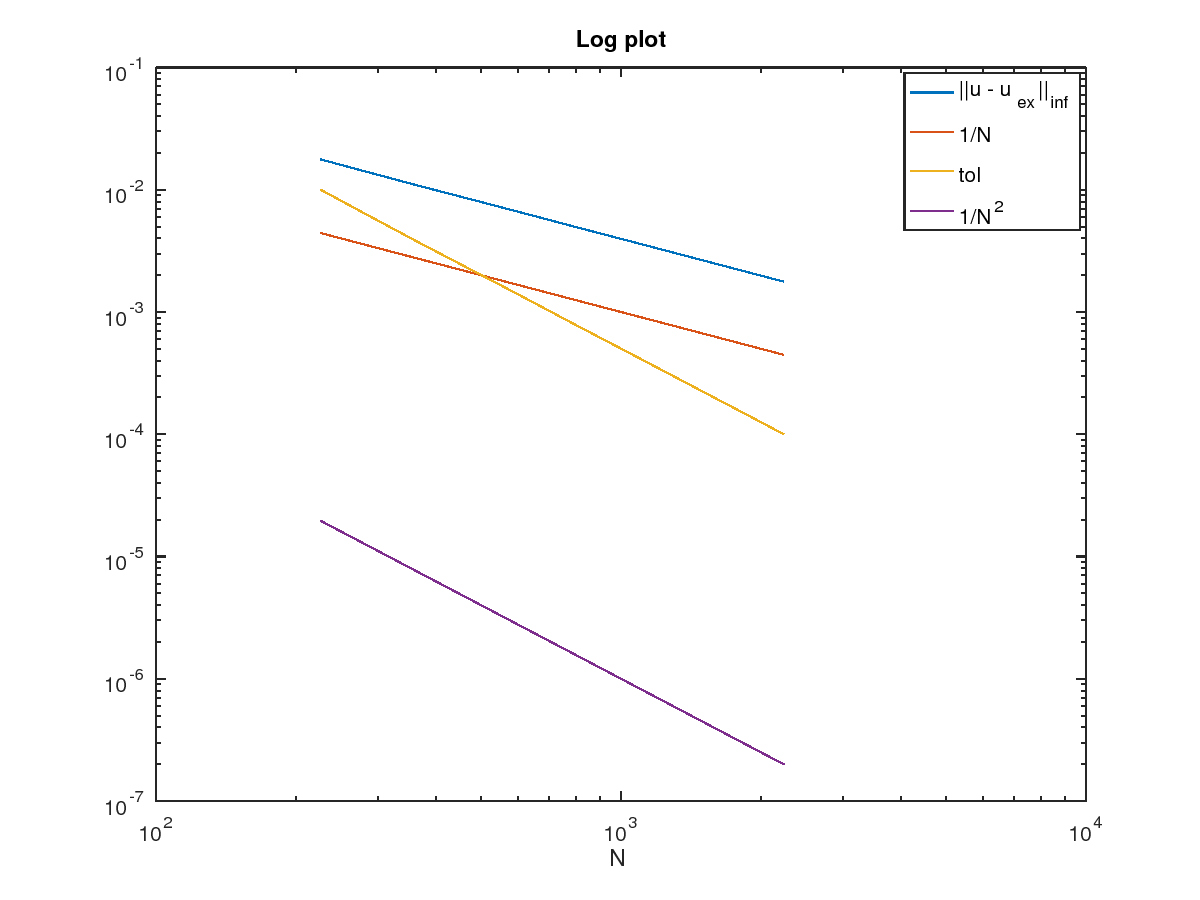
\includegraphics[width=1\linewidth]{time_order}
	\caption[Logarithmic plot of convergence orders is time adaptivity]{The logarithmic plot shows how tolerance , $ tol $, on the difference between the two approximations of the solution, that are numerical solution and initial guess, is of second order respect to $ \frac{1}{N} $, while the error, that is the norm of the difference between exact solution and numerical one, $|| u -u _{ex}||_{\infty}$, is of order one. That means that if an accuracy of $ 0.01 $ is required, then $tol$ has to be equal to $ 0.01^2 $ and, consequently, $ 100 $ time steps will be computed. }
	\label{time_order}
\end{figure}
\section{Space discretization}
The mesh that we decided to use has the quadtrees' numeration for the nodes (see \cite{p4est}). Before going in more details, we will discuss about some difficulties that we have encountered. \\
In view of the fact that we have to solve nonlinear systems, we used the C++ library LIS (Library of Iterative Solvers for linear systems), that, as the name suggests, solves liner problems with iterative methods. Since we needed to implement parallel solving to make the computing time reasonable, we created an interface for LIS, \texttt{lis\_distributed\_class}, in the library that we used for our implementations, called BIM, that manage a "decentralized" parallelization. This means that if we consider a linear system $ A u = f $, each processor will have  only his piece of $ A $, $ u $ and $ f $. In particular LIS requires matrix $ A $ to be divided in strictly separated ranges of rows. Also vectors $ u $ and $ f $ have to be divided among processors with the same ranges. The point is that the numeration that we have chosen for the mesh, does not divide matrix and vectors as LIS requires in a parallel environment. \\
Let see what happens and how we handled with it.
\subsection{Numeration of quadtrees meshes}
As we said above, solver LIS requires to have the matrix $ A $ divided by rows whenever it is asked parallel solving. For example, if we have a matrix with dimension $ 25 \times 25 $ and we want to parallelize it with 2 processors, then the first processor will have the first 15 rows, while the second one the others 10. \\
Let see how the numeration with quadtrees works for an uniform mesh. Just to fix the ideas, imagine to have a mesh of $ 4 \times 4 $ quadrants, that is $ 5 \times 5 $ nodes. The numeration starts form the first quadrant of the first row from the top down and it is done in this order: \\
\begin{center}
	\begin{tikzpicture}[
	squarednode/.style={rectangle, draw=red!60, fill=red!5, thick, minimum size=6mm},
	]
	\centering
	
	%Nodes
	\node[squarednode]      (nodo1)                              {0};
	\node[squarednode]        (nodo2)       [right=of nodo1] {1};
	\node[squarednode]      (nodo3)       [below=of nodo1] {2};
	\node[squarednode]        (nodo4)       [right=of nodo3] {3};
	
	%Lines
	\draw[->] (nodo1.east) -- (nodo2.west);
	\draw[->] (nodo2.west) -- (nodo3.east);
	\draw[->] (nodo3.east) -- (nodo4.west);
	\end{tikzpicture}
\end{center}
Nodes in all quadrants are numerated with this order and also the sequence of quadrants that are taken has the same logic, as is shown in Figure \ref{mesh5x5}. With this procedure the final numeration of all the nodes of a $ 5 \times 5 $  mesh results to be the one in Figure \ref{nodimesh5x5}.
\begin{figure}[h]
	\centering
	\includegraphics[width=0.7\linewidth]{mesh5x5}
	\caption[Sequence of quadrants taken with quadtrees numetation for a mesh $ 5\times 5 $]{Sequence of quadrants taken to be numerated}
	\label{mesh5x5}
\end{figure}

\begin{figure}[h]
	
	\centering
	\includegraphics[width=0.7\linewidth]{nodimesh5x5}
	\caption[Quadtrees numeration of nodes for a mesh $ 5 \times 5 $]{Quadtrees numeration of a $ 5 \times 5 $ mesh}
	\label{nodimesh5x5}
\end{figure}
With a mesh of this dimension, in discrete approximation all the space variables, will turn into  vectors of $ 5^2 = 25 $ components. Therefore the linear system that we have to solve has the shape $ A u = f $, with $ A \in \mathbb{R}^{25} \times \mathbb{R}^{25} $ and  $ u,f \in \mathbb{R}^{25} $. Since our system is coming from advection-diffusion-reaction equations, the most general pattern that matrix $ A $ can have is the one implemented by the method  called \texttt{bim2a\_structure (tmsh, A)} of class \texttt{sparse\_matrix}. This pattern is supposed to compare each node with all its four neighbours, because the problem has diffusion term and, indeed $ A $ has to contain also the discrete gradient of the variable $ u $. For example, in row 6, the previous method will allocate memory in $ A $, in column 6, 2, 7 and 15.\\
If we decide to solve the system with more processors, for example two, then the mesh in Figure \ref{nodimesh5x5} will be split in two parts. All the first 8 quadrants with their nodes will be of processor 1, and the other 8 will go to processor 2. Shared nodes, also called local nodes, that is nodes on the border of quadrants belonging to different processors, will be owned by the first processor that "touches" them. Therefore, in our example nodes 6, 7, 8, 13 and 14, will be owned by processor 1. But then, what happens to the matrix $ A $ ? Each processor will have only cells of the global matrix that link nodes owned by that processors or shared. In our case, processor 1 will have those cells of $ A $ that have indexes less or equal to the number of the last node owned by it, that is node 14. So, it will not have, for example, cells (14,22) or (6,15), that are actually present in rows 14 and 6 in the global matrix.
Figure \ref{patterndivision} shows how the patter of the global matrix is divided, in particular blu elements are of processor 1 while red of processor 2. As we can see there are overlaps that are all the red elements in the processor 1 's region. In fact, in those positions, both processors have their contribution, and to obtain the values of the global matrix, we have to sum them.\\
\begin{figure}[h]
	
	\centering
	\includegraphics[width=0.7\linewidth]{pattern_division}
	\caption[Patter of a matrix come from a mesh $ 5 \times 5 $ ]{It is illustrated the pattern of global matrix $ A $, blu cells are owned by processor 1 and red by processor 2. Where we see red elements in the region of processor 1, it means that there are overlaps, both processors has a value for that cells, and the sum of them gives the value of the global matrix. From this plot is clear that the division of a mesh with quadtrees numerations among processors is not made row by row, as LIS requires. }
	\label{patterndivision}
\end{figure}
The point of this introduction of quadtrees mesh, actually, is to show that the natural separation among processors of the mesh's regions, so of A, is not divided by rows, and there are even overlaps for same elements. Having said that, we already know that LIS wants matrix $ A $ to be strictly separated by rows, so our next aim was to create a new version of the already existing class in BIM of sparse matrices called \texttt{sparse\_matrix}, that handles this problem.
\subsection{Parallelization on the mesh}
\subsubsection{Sparse matrix distributed class}
In this section, we present the alternative of class \texttt{sparse\_matrix}, that was created to allow each processor to assemble its matrix as LIS solver requires. This class is called \texttt{distributed\_sparse\_matrix} and its main variables are the following. 
\\
\\
\begin{lstlisting}[language=C++, caption={class distributed\_sparse\_matrix}]
class
distributed_sparse_matrix
: public sparse_matrix
{
private :
void
non_local_csr_index ();
void
non_local_csr_value ();
size_t is, ie;
MPI_Comm comm;
int mpirank, mpisize;
int nnz_owned;
struct
non_local_t
{
std::vector<int> prc_ptr, row_ind, col_ind;
std::vector<double> a;
} non_local;
std::map<int, std::vector<int>> row_buffers;
std::map<int, std::vector<int>> col_buffers;
std::map<int, std::vector<double>> val_buffers;
std::vector<int> ranges;
std::vector<int> rank_nnz;
public :
void
set_ranges (size_t is_, size_t ie_, MPI_Comm comm_ =     
MPI_COMM_WORLD);
distributed_sparse_matrix (size_t is_, size_t ie_,
MPI_Comm comm_= MPI_COMM_WORLD)
: mapped (false)
{ set_ranges (is_, ie_, comm_); }
distributed_sparse_matrix (MPI_Comm comm_ = MPI_COMM_WORLD)
: comm (comm_), mapped (false)
{ }
\end{lstlisting}

Let $ A $ be a matrix of type \texttt{distributed\_sparse\_matrix}. First of all, we have to set variables \texttt{is} and \texttt{ie}, which indicate the first and the last row owned by the current rank. These are computed in \texttt{lis\_distributed\_class} and passed to $ A $ by a method in the following way: \texttt{A.set\_ranges (is, ie)}. This sets also the components of \texttt{ranges}, that is the rows' ranges in which the global matrix is divided among the processors.\\
In lines 15-19 it is defined the structure \texttt{non\_local} that has \texttt{prc\_ptr}, a vector supposed to contain the numbers of nonzero elements that local A has in each range. Differently from vector \texttt{ranges}, \texttt{prc\_ptr}, like all the others, changes from rank to rank; indeed each rank has a different $ A $. So this is a way to indicate how many elements and to who the current rank has to communicate. The other vectors in \texttt{non\_local} are basically the indexes and values in AIJ format of the elements of A out of the range of current rank. All of them are computed by \texttt{non\_local\_csr\_index}. 
\begin{lstlisting}[language=C++, caption={distributed\_sparse\_matrix::non\_local\_csr\_index ()}]
void
distributed_sparse_matrix::non_local_csr_index ()
{
non_local.row_ind.clear ();
non_local.col_ind.clear ();
non_local.a.clear ();
this->set_properties ();
non_local.prc_ptr.assign (this->mpisize + 1, 0);
sparse_matrix::col_iterator jj;
for (size_t ii = 0; ii < this->mpisize; ++ii)
{
non_local.prc_ptr[ii+1] = non_local.prc_ptr[ii];
if (ii != mpirank)
for (size_t kk = ranges[ii]; kk < ranges[ii+1]; ++kk)
{
non_local.prc_ptr[ii+1] += (*this)[kk].size ();
non_local.col_ind.reserve ((*this)[kk].size ());
non_local.row_ind.reserve ((*this)[kk].size ());
for (jj  = (*this)[kk].begin ();
jj != (*this)[kk].end (); ++jj)
{
non_local.row_ind.push_back (kk);
non_local.col_ind.push_back 
(this->col_idx (jj));
non_local.a.push_back (this->col_val (jj));
}
}
}
non_local.a.resize (non_local.row_ind.size ());
}
\end{lstlisting}
As we see, \texttt{prc\_ptr} is, actually, the cumulative sum of the number of nonzero elements in the others ranges. We also see that with the check in line 13, only out-of-range elements are considered.\\
Up to now, for each $ A $ implemented by different ranks, we can identify which elements of the matrix are out of the current processor's range and to which range they below, therefore to which rank they have to be communicated. Going back to Figure \ref{patterndivision} and taking the ranges $ (0,14) $ for rank 0 and $ (15,25) $ for rank 1, matrix $ A $ of rank 0 will have empty vectors in \texttt{non\_local} structure, because its elements are all in the current range, while rank 1 will have \texttt{non\_local} vectors of size 18, since this is the number of its elements that stay in rank 0 's range. Now the aim is to communicated these components to rank 0.
\begin{lstlisting}[language=C++, caption={distributed\_sparse\_matrix::remap ()}]
void
distributed_sparse_matrix::remap ()
{
non_local_csr_index ();
/// Distribute buffer sizes
rank_nnz.assign (mpisize, 0);
for (int ii = 0; ii < mpisize; ++ii)
rank_nnz[ii] = non_local.prc_ptr[ii+1] 
- non_local.prc_ptr[ii];
MPI_Alltoall (MPI_IN_PLACE, 1, MPI_INT, &(rank_nnz[0]), 1,
MPI_INT, comm);
/// Allocate buffers
for (int ii = 0; ii < mpisize; ++ii)
if ((rank_nnz[ii] > 0) && (ii != mpirank))
{
row_buffers[ii].resize (rank_nnz[ii]);
col_buffers[ii].resize (rank_nnz[ii]);
val_buffers[ii].resize (rank_nnz[ii]);
}
/// Communicate overlap regions
/// 1) communicate row_ptr
std::vector<MPI_Request> reqs;
for (int ii = 0; ii < mpisize; ++ii)
{
if (ii == mpirank) continue; // No communication to self!
if (rank_nnz[ii] > 0) // we must receive 
//something from rank ii
{
int recv_tag = ii   + mpisize * mpirank;
reqs.resize (reqs.size () + 1);
MPI_Irecv (&(row_buffers[ii][0]), row_buffers[ii].size (),
MPI_INT, ii, recv_tag, comm, &(reqs.back ()));
}
int rank_nnz_snd_ii = non_local.prc_ptr[ii+1] -
non_local.prc_ptr[ii];
if (rank_nnz_snd_ii > 0) // we must send something to rank ii
{
int send_tag = mpirank + mpisize * ii;
reqs.resize (reqs.size () + 1);
MPI_Isend (&(non_local.row_ind[non_local.prc_ptr[ii]]),
rank_nnz_snd_ii, MPI_INT, ii, send_tag, comm,
&(reqs.back ()));
}     
}
MPI_Waitall (reqs.size (), &(reqs[0]), MPI_STATUSES_IGNORE);
reqs.clear ();
/// 2) communicate col_ind
for (int ii = 0; ii < mpisize; ++ii)
{
if (ii == mpirank) continue; // No communication to self!
if (rank_nnz[ii] > 0) // we must receive 
// something from rank ii
{
int recv_tag = ii   + mpisize * mpirank;
reqs.resize (reqs.size () + 1);
MPI_Irecv (&(col_buffers[ii][0]), col_buffers[ii].size (),
MPI_INT, ii, recv_tag, comm, &(reqs.back ()));
}
int rank_nnz_snd_ii = non_local.prc_ptr[ii+1] -
non_local.prc_ptr[ii];
if (rank_nnz_snd_ii > 0) // we must send 
// something to rank ii
{
int send_tag = mpirank + mpisize * ii;
reqs.resize (reqs.size () + 1);
MPI_Isend (&(non_local.col_ind[non_local.prc_ptr[ii]]),
rank_nnz_snd_ii, MPI_INT, ii, send_tag, comm,
&(reqs.back ()));
}     
}
MPI_Waitall (reqs.size (), &(reqs[0]), MPI_STATUSES_IGNORE);
reqs.clear ();
mapped = true;
update = true;
}
\end{lstlisting}
Here we encounter \texttt{row\_buffers}, \texttt{col\_buffers} and \texttt{val\_buffers} that basically are containers of the elements that the current rank receives from the others. The numbers of these elements are set in the vector \texttt{rank\_nnz} with \texttt{MPI\_Alltoall} (lines 7-12). With this numbers, we set buffers' sizes . \\
Now comes the crucial part, in which each rank sends the indexes of its non local elements and receives the others' non local elements that are in its range. With line 25, communication to itself is avoided and the procedure of sending and receiving is done only if actually there is some thing to send or receive. Therefore, essentially, \texttt{distributed\_sparse\_matrix::remap ()} set the indexes of the cells in $ A $ in which each processor has to receive a value. For the communication of these values, we made the next method.
\begin{lstlisting}[language=C++, caption={distributed\_sparse\_matrix::assemble ()}]
void
distributed_sparse_matrix::assemble ()
{
if (! mapped)
remap ();
non_local_csr_value ();
/// 3) communicate values
std::vector<MPI_Request> reqs;
for (int ii = 0; ii < mpisize; ++ii)
{
if (ii == mpirank) continue; // No communication to self!
if (rank_nnz[ii] > 0) // we must receive something 
// from rank ii
{
int recv_tag = ii   + mpisize * mpirank;
reqs.resize (reqs.size () + 1);
MPI_Irecv (&(val_buffers[ii][0]), val_buffers[ii].size (),
MPI_DOUBLE, ii, recv_tag, comm, &(reqs.back
()));
}
int rank_nnz_snd_ii = non_local.prc_ptr[ii+1] -
non_local.prc_ptr[ii];      
if (rank_nnz_snd_ii > 0) // we must send something 
// to rank ii
{
int send_tag = mpirank + mpisize * ii;
reqs.resize (reqs.size () + 1);
MPI_Isend (&(non_local.a[non_local.prc_ptr[ii]]),
rank_nnz_snd_ii, MPI_DOUBLE, ii, send_tag,
comm, &(reqs.back ()));
}     
}
MPI_Waitall (reqs.size (), &(reqs[0]), MPI_STATUSES_IGNORE);
reqs.clear ();
/// 4) insert communicated values into sparse_matrix
for (int ii = 0; ii < mpisize; ++ii) // loop over ranks
if (ii != mpirank)
for (int kk = 0; kk < rank_nnz[ii]; ++kk)  
(*this)[row_buffers[ii][kk]][col_buffers[ii][kk]]
+= val_buffers[ii][kk];
/// 5) zero out communicated values  
for (int iprc = 0; iprc < mpisize; ++iprc)
if (iprc != mpirank)
{
for (int ii = non_local.prc_ptr[iprc];
ii < non_local.prc_ptr[iprc+1]; ++ii)
// the following will throw if we try to access
// an element which does not exist yet!
(*this)[non_local.row_ind[ii]].at (non_local.col_ind[ii])
= 0.0;
}
if (update)
{
nnz_owned = 0;
for (int irow = is; irow < ie; ++irow)
nnz_owned += (*this)[irow].size ();
}
update = false;
}
\end{lstlisting}
In nonlinear solving of partial differential equations problems, often, pattern of the matrix $ A $ remains the same for all the nonlinear and, eventually, time steps. This is why we actually separated the communications of the indexes from the one of the values; indeed, ones computed, \texttt{row\_buffers} and \texttt{col\_buffers} are supposed to remain the same, therefore there is no need to calculate them every time. Actually, the same is true also for the \texttt{non\_local} structure of $ A $. This is why we implemented also the method \texttt{non\_local\_csr\_value ()}, that updates only the values of \texttt{non\_local.a}. Regarding the buffers, communication of the values is essentially the same as before and, it is in lines 36-40, that the communicated values are inserted in matrix $ A $. At the end all the out-of-range values of $ A $ are set to zero.\\
\subsubsection{Distributed vector class}
In our example of linear system $ Au = f $, we know that every rank has his own matrix $ A $ and that the sum of all of them represents the global matrix. Since $ (A_1 + A_2) (u_1 + u_2) \neq A_1 u_1 + A_2 u_2$, $ u $ has to have the global values, but it is enough to allocate the ones that correspond to owned and shared nodes, and not to all the nodes, since $ A $ has nonzero elements only for these nodes. On the other hand, $ f $ could have elements different from zero only where $ A $ has nonzero rows, that is in all owned and shared nodes. But, again, if we want to pass this vectors in LIS for parallel solving, we have to pass just the piece of the current range, and it means that all the out-of-range values has to bo communicated to their correspondent processors.
For this regard, we implemented a new class called \texttt{distributed\_vector}. Let see how is structured.
\begin{lstlisting}[language=C++, caption={distributed\_vector class}]
class
distributed_vector
{
private:
MPI_Comm comm;
int mpirank;
int mpisize;
bool mapped;
int owned_count;
int is, ie;
/// vector entries owned by the current node
std::vector<double> owned_data;
/// vector entries touched by the current node
/// that belong somwhere else
std::map<int, double> non_local_data;
/// Structure to hold data of ghost entries
/// in a format amenable for send/receive
struct
ghosts_t
{
std::vector<int> prc_ptr, row_ind, rank_nnz;
std::vector<double> a;
} ghosts;
/// Copy data from non_local_data to ghosts
void
ghost_csr ();
/// Update ghosts.
void
ghost_csr_update ();
/// Structure to hold data of ghost entries
/// in a format amenable for send/receive
struct
mirrors_t
{
std::vector<int> prc_ptr, row_ind, rank_nnz;
std::vector<double> a;
} mirrors;
/// the entries that are owned by rank i
/// are numbered between ranges[i]
/// and ranges[i+1]
std::vector<int> ranges;
/// check whether the idx-th global
/// entry is owned by the current rank
inline bool
is_owned (int idx) const
{ return idx >= is && idx < ie; }
/// check whether the idx-th global
/// entry is owned by the given rank
inline bool
is_owned (int idx, int irank) const
{ return idx >= ranges[irank] && idx < ranges[irank+1]; }
/// return the rank that owns the idx-th entry
inline int
owner (int idx)
{
auto ir = std::lower_bound (ranges.begin (), 
ranges.end (), idx);
return int ((ir - ranges.begin ()) - 1);
}
public:
distributed_vector (int owned_count_,
MPI_Comm comm_ = MPI_COMM_WORLD);
distributed_vector (int is_, int ie_,
MPI_Comm comm_ = MPI_COMM_WORLD);
distributed_vector () {};
void
set_owned_count (int owned_count_, MPI_Comm comm_ =  
MPI_COMM_WORLD);
\end{lstlisting}
First of all, let have a look at the constructors. Suppose to have a distributed vector $ u $, when we declare it, we have also to provide either the dimension or the extremes of the owned nodes' range. If it is not possible, because, for example we are declaring this kind of vectors in a class that does not have this information internally, then we can declared it without anything, but when we want to use really that vector, we must implement first \texttt{u.set\_owned\_count (dimension\_range)}. This is because the first two constructors and that method set the size of \texttt{owned\_data}, which with \texttt{non\_local\_data}, is the main container of the class. Indeed, the first one is meant to contain values of the owned nodes, so the values that ere in the range of the current rank. The second will contain eventually the values and their indexes of out-of-range elements. Structures \texttt{ghosts} and \texttt{mirrors} has the same role as \texttt{non\_local} and \texttt{buffers} in \texttt{distributed\_sparse\_matrix}. The first one, that contains the non local elements, is computed  with private method \texttt{ghosts\_csr ()}, while the second one is computed after the communications done in methods called \texttt{remap ()} and \texttt{assemble ()}, analogue at the ones of the matrix's class, and contains the elements that are in the current range and are sent from the other ranks. All the mechanism of sending and receiving is very similar to the one shown in the previous section, so we will limit ourselves to recall the main steps. 
\begin{enumerate}
	\item  copy \texttt{non\_local\_data} into ghosts structure;
	\item  send ghosts indexes and receive into mirrors;
	\item add mirrors into \texttt{owned\_data};
	\item copy \texttt{owned\_data} into mirrors;
	\item send mirrors data and receive into ghosts;
	\item copy ghosts data into non\_local\_data.
\end{enumerate}
The two first steps are of the method \texttt{remap ()}, while the others are in \texttt{assemble ()}. Besides, steps 4, 5 and 6 were not present in the previous class. They are a kind of inverse communication, indeed after the update of \texttt{owned\_data}, this one is communicated to the others' \texttt{non\_local\_data}. In this way, we ensure that also \texttt{non\_local\_data} will be updated with the global values. This needs to happen because, as we said before, $ u $ has to have the global values also out-of-the range.\\
The use of objects of this class is quite easy since is sufficient to write \texttt{u[i] = val} and, if  \texttt{i} belong to the current range, then it is equivalent to write \texttt{owned\_data[i] = val}, otherwise it is inserted a new component \texttt{<i, val>} in the map \texttt{non\_local\_data}, or it is updated, if one exists already with this index. It is enough to initialize all the elements out-of-range that we are interested to keep inside $ u $, and then they will be always updated with \texttt{assemble ()}. In our case, they will be the shared nodes.\\
\subsection{Ordering of more fields on the same mesh}
Now we have to specify how the presence of two fields, as it is in our test problem \eqref{tumor_system} in Chapter 1, can be handled with the parallelization. \\
In our computational environment we keep the fields, $ m $ and $ n $, in the same container, that in this case will have twice the mesh size. The same is true for all the other vectors, like the initial guess or the right-hand-side of the system.\\
Consequently we can imagine a partition as the one in Figure \ref{A_m_n}, with $ N $ number of nodes. This can be useful when we, for example, implement the matrix; indeed, generally, the four blocks are done separately. But since our parallelization is based on the mesh's quadrants, we decided to weave the two fields $ m $ and $ n $, which means that vectors will be ordered by nodes. Starting from the first node, all the variables evaluated in it are listed before passing to the second node and so on. Figure \ref{weave} shows the idea of this ordering, of course all the structure of $ A $ will be different from the one in Figure \ref{A_m_n}, but we can still treated $ A $ as separated in 4 blocks, even if it is not, using variables of type \texttt{ordering} that pick the cells of the matrix that belongs to one of the blocks.
\begin{figure}[h]
	\centering
	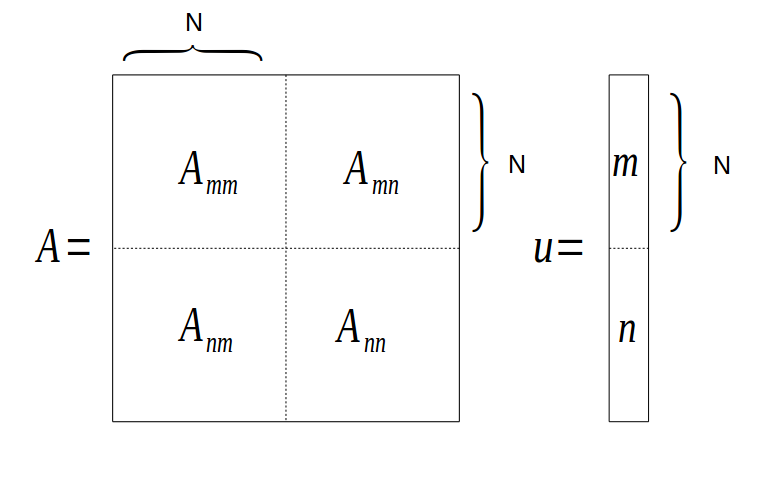
\includegraphics[width=0.7\linewidth]{A_m_n}
	\caption[Partition of matrix and vectors among $ m $ and $ n $]{Partition of matrix and vectors among $ m $ and $ n $, with $ N $ the number of nodes. This is a intuitive division, but is not going to be the chosen one because we want to order by nodes and not by fields. Nevertheless this is a useful way to imagine it; indeed when we compute the matrix, we will do it with each block separately. For working with the matrix as it is structure in this way, even if it is no, we implemented variables of type \texttt{ordering} that do this job. }
	\label{A_m_n}
\end{figure}
\begin{figure}[h]
	\centering
	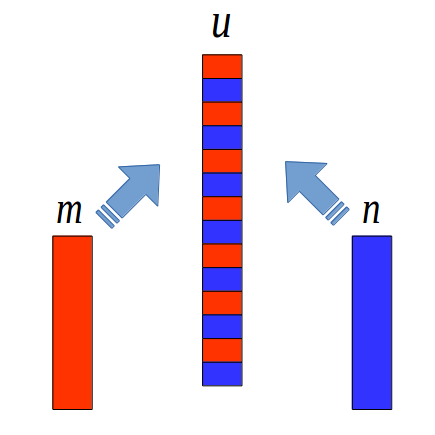
\includegraphics[width=0.7\linewidth]{weave}
	\caption[Chain of different fields]{This illustrates how the two field, $ m $ and $ n $, are weaved node after node in order to preserve the division by quadrants in parallel computing.}
	\label{weave}
\end{figure}
 